\part{Planning prévisionnel}

\section{Étapes du projets}

Notre projets comporte 4 étapes principales. Chacune de ces étapes aura une date de remise définie des le debut du projet. 

\paragraph{La rédaction du cahier des charges}

Dans cette étape nous avons eu principalement besoin de rédiger la demande du client. 
Nous avons aussi eu à étudier le fonctionnement du logiciel Royal que l'on a choisi d'ameliorer afin d'arriver au but visé.
Les contraintes liées à l'amélioration de ce logiciels nous permettent de definire la faisabilité des differentes fonctions. 

\paragraph{La rédaction du dossier d'analyse}

Dans cette étape nous aurons à approfondir l'analyse ainsi que la conception des différentes fonctions ainsi que le fonctionnement du logiciel Royal. 
Nous définirons aussi les différents outils utilisé afin de développer le projet tels que 
Eclipse \footnote{Site de l'IDE Eclipse : http://www.eclipse.org/} 
pour le developpement JAVA ou encore 
PowerAMC \footnote{Site officiel de PowerAMC : http://www.sybase.fr/products/modelingdevelopment/poweramc}
pour la réalisation des MCD.

\paragraph{La réalisation d'un premier prototype}

Afin de rendre un prototype, le 5 Décembre 2011, répondant aux principales demandes de l'utilisateur nous développerons les fonctions de priorités 1 et 2.
Pour permettre l'implémentation de certaines de ces fonctions, nous aurons à modifier la base de données en suivant le models modifié dans l'étape précédente.  

\paragraph{La finalisation du projet}

Cette étape sera la dernière de notre projet et devra être effectuée avant le 19 Janvier 2012 (date de livraison de notre projet).
Pour cette étape nous développerons les fonctions de priorités inférieur afin de répondre à des besoin moins important. 

\section{Éstimation du temps nécessaire}
Pour la réalisation des estimations de temps nécessaire à la réussite de ce projet,
nous nous sommes basé sur deux méthodes. 

La première méthode choisie est l'\emph{éstimation par analogie}.
Elle correspond à se fier à la conception du cahier des charges pour l'estimation du temps que prendra l'intégralité du projet. 

\begin{tabular}{|l l|l|l|}
\hline
&& Durée proportionnelle & Durée concrète \\
\hline
Opportunité & Étude préalable & 10\% & 60h \\
\hline
Élaboration & Conseption de la solution détaillée & 30\% & 180h \\
\hline
Construciton & Développement & 50\% & 300h \\
\hline
Transition & Mise en œuvre & 10\% & 60h \\
\hline
\end{tabular}

Avec cette méthode, nous avons une estimation de travail de $60 + 180 + 300 + 60 = 600$ heures. 

\section{Planification des délais}

Pour la planification des délais, nous avons utilisé la méthode du \emph{diagramme de GANTT}.
\begin{figure}[h]
\begin{center}
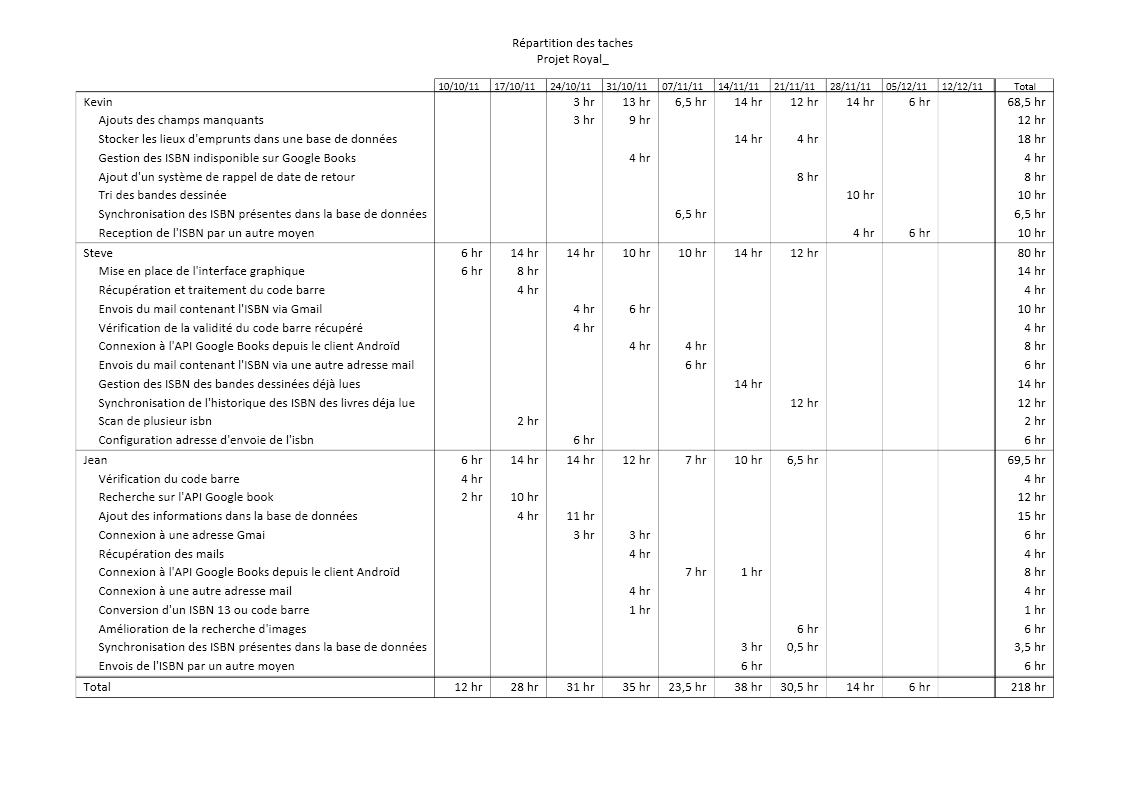
\includegraphics[height=12cm]{../repartition_des_taches.png}
\end{center}
\caption{Éstimation de notre temps de travail}
\end{figure}
